\documentclass{article}

\date{19 novembre 2023}
\usepackage[nb-sem=6, auteurs={Kylian Boyet, George Ober, Félix Rondeau, Elijah Gaillard, Hugo Vangilluwen (relecture)}]{../kholles}

\begin{document}

\maketitle

\begin{question_kholle}{Liens entre le graphe de $f$ et ceux de $g$ et $h$ définies par $g(x)=af(x)$ et $h(x)=f(x+a)$.}
  \hfill\\
  \begin{minipage}{0.5\textwidth}
    \begin{figure}[H]
      \centering
      \begin{tikzpicture}
        \node at (3.3,2.5) {$\mathcal{D}_g=\mathcal{D}_f$};
        \draw [->] (-1,0) -- (4,0);
        \draw [->] (0,-2) -- (0,3);

        \coordinate (A) at (1.5, 2);
        \coordinate (B) at (1.5, -1);

        \draw [dashed, gray] (0, 2) -- (A) -- (1.5,0);
        \draw [dashed, gray] (0, -1) -- (B) -- (1.5,0);

        \fill [radius=1.5pt] (A) circle node[above=2pt] {\small $(x,g(x))$};
        \fill [radius=1.5pt] (B) circle node[below=2pt] {\small $(x,f(x))$};

        \draw[-Stealth, thick] (1.7,-1) arc (-90:90:1.5) node [midway, right] {$\bm{\times a}$};

        \draw (1.5,-0.05) -- (1.5,0.05) node[fill=white, above] {\footnotesize $x$};
        \draw (-0.05,2) -- (0.05,2) node[left, xshift=-3mm] {\footnotesize $g(x)$};
        \draw (-0.05,-1) -- (0.05,-1) node[left, xshift=-3mm] {\footnotesize $f(x)$};
      \end{tikzpicture}
      \caption{Lien entre le graphe de $f$ et de $g$.}
    \end{figure}
  \end{minipage}
  \begin{minipage}{0.5\textwidth}
    \begin{figure}[H]
      \centering
      \begin{tikzpicture}
        \node at (2.5,3.5) {$\mathcal{D}_h=\{x-a\mid x\in\mathcal{D}_f\}$};
        \draw [->] (-1,0) -- (5,0);
        \draw [->] (0,-1) -- (0,4);

        \coordinate (A) at (1.2, 2);
        \coordinate (B) at (3.5, 2);

        \draw (1.2,-0.05) -- (1.2,0.05) node[below, yshift=-1mm] {\footnotesize $x$};
        \draw (3.5,-0.05) -- (3.5,0.05) node[below, yshift=-1mm] {\footnotesize $x+a$};
        \draw (-0.05,2) -- (0.05,2) node[left, xshift=-3mm] {\footnotesize $f(x+a)$};

        \draw [dashed, gray] (0,2) -- (A) -- (1.2, 0);
        \draw [dashed, gray] (0,2) -- (B) -- (3.5, 0);

        \fill [radius=1.5pt] (A) circle node[above=2pt] {\small $(x,h(x))$};
        \fill [radius=1.5pt] (B) circle node[below=2pt, fill=white] {\small $(x+a, f(x+a))$};

        \draw (A) node [below=1ex, white, fill=white] {a}; % TODO: Dirty fix. Change it.
        \draw [-Stealth, thick] (B) -- (A) node [below] {$\bm{-a}\vv{\bm{i}}$};
      \end{tikzpicture}
      \caption{Lien entre le graphe de $f$ et de $h$.}
    \end{figure}
  \end{minipage}
\end{question_kholle}

\begin{question_kholle}{Liens entre le graphe de $f$ et ceux de $g$ et $h$ définies par $g(x)=f(ax)$ et $h(x)=f(a-x)$.}
  \hfill\\
  \begin{minipage}{0.5\textwidth}
    \begin{figure}[H]
      \centering
      \begin{tikzpicture}
        \node at (2.5,3.5) {$\mathcal{D}_g=\left\{\frac{x}{a}\mid x\in\mathcal{D}_f\right\}$};
        \draw [->] (-1,0) -- (5,0);
        \draw [->] (0,-1) -- (0,4);

        \coordinate (A) at (1.2, 2);
        \coordinate (B) at (3.5, 2);

        \draw (1.2,-0.05) -- (1.2,0.05) node[below, yshift=-1mm] {\footnotesize $x$};
        \draw (3.5,-0.05) -- (3.5,0.05) node[below, yshift=-1mm] {\footnotesize $ax$};
        \draw (-0.05,2) -- (0.05,2) node[left, xshift=-3mm] {\footnotesize $f(ax)$};

        \draw [dashed, gray] (0,2) -- (A) -- (1.2, 0);
        \draw [dashed, gray] (0,2) -- (B) -- (3.5, 0);

        \fill [radius=1.5pt] (A) circle node[above=2pt] {\small $(x,g(x))$};
        \fill [radius=1.5pt] (B) circle node[above=2pt] {\small $(ax, f(ax))$};

        \draw [-Stealth, thick] (3.5, 1.9) arc (0:-180:1.15) node [midway, above=2pt] {$\bm{\times \frac{1}{a}}$};
      \end{tikzpicture}
      \caption{Lien entre le graphe de $f$ et de $g$.}
    \end{figure}
  \end{minipage}
  \begin{minipage}{0.5\textwidth}
    \begin{figure}[H]
      \centering
      \begin{tikzpicture}
        \draw [->] (-1,0) -- (5,0);
        \draw [->] (0,-1) -- (0,4);

        \coordinate (A) at (0.8, 2);
        \coordinate (B) at (3.7, 2);

        \draw [dashed, gray] (0,2) -- (A) -- (0.8, 0);
        \draw [dashed, gray] (0,2) -- (B) -- (3.7, 0);

        \fill [radius=1.5pt] (A) circle node[above=2pt] {\small $(x,h(x))$};
        \fill [radius=1.5pt] (B) circle node[above=2pt] {\small $(a-x, f(a-x))$};

        \draw [thick, dashed] (2.25, -1) -- (2.25, 3.5);

        \draw (0.8,-0.05) -- (0.8,0.05) node[below, yshift=-1mm] {\footnotesize $x$};
        \draw (3.7,-0.05) -- (3.7,0.05) node[below, yshift=-1mm] {\footnotesize $a-x$};
        \draw (2.25,-0.05) -- (2.25,0.05) node[below, yshift=-1mm, fill=white] {\footnotesize $\frac{a}{2}$};
        \draw (-0.05,2) -- (0.05,2) node[left, xshift=-3mm] {\footnotesize $f(a-x)$};

        \node [fill=white] at (2.5,3.5) {$\mathcal{D}_g=\{a-x \mid x\in\mathcal{D}_f\}$};
      \end{tikzpicture}
      \caption{Lien entre le graphe de $f$ et de $h$.}
    \end{figure}
  \end{minipage}
\end{question_kholle}

\pagebreak

\begin{question_kholle}{Présentation exhaustive de la fonction $\arccos$.}

  Premièrement, ladite fonction est la bijection réciproque de la fonction $\bigl.\cos\bigr|_{[0,\pi]}^{[-1,1]}$. D'où :
  \[
    \arccos = \left|
    \begin{array}{rcl}
      [-1,1] & \to     & [0 , \pi]                                                 \\ [1ex]
      x      & \mapsto & \left( \bigl.\cos\bigr|_{[0,\pi]}^{[-1,1]}\right)^{-1}(x)
    \end{array}
    \right.
  \]
  Ainsi, pour $x\in [-1,1]$, $\arccos (x)$ est l'unique solution de l'équation d'inconnue $\theta \in \textstyle [0 ,\pi]$, \[\cos(\theta) = x\].

  \noindent Il découle alors naturellement des propriétés héréditairement acquises de $\bigl.\cos\bigr|_{[0,\pi]}^{[-1,1]}$ :

  \begin{enumerate}
    \item $\arccos$ est strictement décroissante sur $[-1,1]$.
    \item $\arccos \in \mathcal{C}^0\left([-1,1],[0 , \pi] \right)$.
    \item $\arccos \in \mathcal{D}^1\left(]-1,1[,]0 ,\pi [ \right)$.
    \item $\displaystyle\arccos'(x) = -\frac{1}{\sqrt{1-x^2}}$ pour tout $x\in]-1,1[$.
    \item $\arccos$ admet deux demi-tangentes verticales en $-1$ et $1$.
  \end{enumerate}

  \

  Graphe de $\arccos$ :
  \begin{figure}[H]
    \centering
    \begin{tikzpicture}[scale=2]
      \draw [->] (-1.5,0) -- (pi+0.5,0);
      \draw [->] (0,-1.5) -- (0,pi+0.5);

      \draw (1,-0.05) -- (1,0.05) node[below, yshift=-3mm] {\footnotesize $1$};
      \draw (-1,-0.05) -- (-1,0.05) node[below, yshift=-3mm] {\footnotesize $-1$};
      \draw (pi/2,-0.05) -- (pi/2,0.05) node[below, yshift=-3mm] {\footnotesize $\frac{\pi}{2}$};
      \draw (pi,-0.05) -- (pi,0.05) node[below, yshift=-3mm] {\footnotesize $\pi$};

      \draw (-0.05,1) -- (0.05,1) node[left, xshift=-3mm] {\footnotesize $1$};
      \draw (-0.05,-1) -- (0.05,-1) node[left, xshift=-3mm] {\footnotesize $-1$};
      \draw (-0.05,pi/2) -- (0.05,pi/2) node[left, xshift=-3mm] {\footnotesize $\frac{\pi}{2}$};
      \draw (-0.05,pi) -- (0.05,pi) node[left, xshift=-3mm] {\footnotesize $\pi$};

      \draw[thick, domain=0:pi, smooth, variable=\x, lime] plot ({\x}, {cos(\x*180/pi)});
      \draw[thick, domain=-1:1, samples=100, variable=\x, purple] plot ({\x}, {pi*acos(\x)/180});
      \draw[thick, domain=-1:pi, smooth, variable=\x, teal] plot ({\x}, {\x});
      \draw[dashed, thick, domain=-1.5:pi, smooth, variable=\x, gray] plot ({\x}, {pi/2-\x}) node[left, xshift=1cm, fill=white] {$y=\frac{\pi}{2}-x$};

      \draw [->] (-1,pi) -- (-1,pi-0.5);
      \draw [->] (1,0) -- (1,0.5);
      \draw [->] (pi,-1) -- (pi-0.5,-1);
      \draw [->] (0,1) -- (0.5,1);
    \end{tikzpicture}
    \caption{$\arccos$ en violet, $\cos$ en vert et la première bissectrice en bleu.}
  \end{figure}
\end{question_kholle}

\pagebreak

\begin{question_kholle}{Présentation exhaustive de la fonction $\arctan$.}
  Premièrement, ladite fonction est la bijection réciproque de la fonction $\bigl. \tan\bigr| _{\left] -\frac{\pi}{2}, \frac{\pi}{2}\right[ }$. D'où :
        \[
          \arctan = \left|\begin{array}{rcl}
            \mathbb{R} & \to     & \left] -\frac{\pi}{2}, \frac{\pi}{2}\right[                                         \\ [1ex]
            x          & \mapsto & \left(\bigl.\tan\bigr|_{\left] -\frac{\pi}{2}, \frac{\pi}{2}\right[}\right)^{-1}(x)
          \end{array}\right.
        \]
        Ainsi, pour $x\in \mathbb{R}$, $\arctan (x)$ est l'unique solution de l'équation d'inconnue $\theta \in \textstyle \left] -\frac{\pi}{2}, \frac{\pi}{2}\right[$,
  \[
    \tan(\theta) = x
  \]
  \noindent Il découle alors naturellement des propriétés héréditairement acquises de $\bigl.\tan\bigr|_{\left] -\frac{\pi}{2}, \frac{\pi}{2}\right[}$ :

  \begin{enumerate}
    \item $\arctan$ est impaire.
    \item $\arctan \in \mathcal{C}^0\left(\mathbb{R},\left] -\frac{\pi}{2}, \frac{\pi}{2}\right[ \right)$.
    \item $\arctan \in \mathcal{D}^1\left(\mathbb{R},\left] -\frac{\pi}{2}, \frac{\pi}{2}\right[ \right)$.
    \item $\displaystyle\arctan'(x) = \frac{1}{1+x^2}$ pour tout $x\in\mathbb{R}$.
  \end{enumerate}

  Graphe de $\arctan$ :
  \begin{figure}[H]
    \centering
    \begin{tikzpicture}[scale=1.5]
      \draw [->] (-pi-0.5,0) -- (pi+0.5,0);
      \draw [->] (0,-pi-0.5) -- (0,pi+0.5);

      \draw (-pi/2,-0.05) -- (-pi/2,0.05) node[below, xshift=-5mm, yshift=-3mm] {\footnotesize $-\frac{\pi}{2}$};
      \draw (pi/2,-0.05) -- (pi/2,0.05) node[below, xshift=-3mm, yshift=-3mm] {\footnotesize $\frac{\pi}{2}$};

      \draw (-0.05,pi/2) -- (0.05,pi/2) node[left, xshift=-3mm, yshift=-5mm] {\footnotesize $\frac{\pi}{2}$};
      \draw (-0.05,-pi/2) -- (0.05,-pi/2) node[left, xshift=-3mm, yshift=-5mm] {\footnotesize $-\frac{\pi}{2}$};

      \draw[thick, domain=-pi-0.5:pi+0.5, samples=100, variable=\x, purple] plot ({\x}, {pi*atan(\x)/180});
      \clip(-pi-0.5,-pi-0.5) rectangle (pi+0.5,pi+0.5);
      \draw[thick, domain=-pi/2+0.25:pi/2-0.25, smooth, variable=\x, lime] plot ({\x}, {tan(\x*180/pi)});
      \draw[thick, domain=-pi:pi, smooth, variable=\x, teal] plot ({\x}, {\x});

      \draw[dashed, thick, gray] (-pi-0.5, pi/2) -- (pi+0.5,pi/2);
      \draw[dashed, thick, gray] (-pi-0.5, -pi/2) -- (pi+0.5,-pi/2);
      \draw[dashed, thick, gray] (pi/2, -pi-0.5) -- (pi/2, pi+0.5);
      \draw[dashed, thick, gray] (-pi/2, -pi-0.5) -- (-pi/2, pi+0.5);
    \end{tikzpicture}
    \caption{$\arctan$ en violet, $\tan$ en vert et la première bissectrice en bleu.}
  \end{figure}
  On a aussi (visible sur le graphe) :
  \[
    \forall x \in \mathbb{R}_+, \quad \arctan(x) \leq x.
  \]

  Et enfin : % TODO: Graphe
  \[
    \forall x \in \mathbb{R}^*, \quad \arctan(x) + \arctan \left( \frac{1}{x} \right) =
    \left\{ \begin{array}{cl}
      \frac{\pi}{2}  & \text{si } x \ > \ 0  \\
      -\frac{\pi}{2} & \text{si } x \ < \ 0.
    \end{array} \right.
  \]

\end{question_kholle}

\begin{question_kholle}{2 preuves de $\arcsin(x) + \arccos(x) =\frac{\pi}{2}$ sur $[-1,1]$, dont une basée sur une interprétation géométrique du cercle trigonométrique.}
  On remarque sur la \autoref{sem6:q4:1} que la droite d'équation polaire $\displaystyle\theta=\frac{\pi}{4}$ est axe de symétrie de la figure. On a donc
  \[
    \frac{\arcsin x+\arccos x}{2} = \frac{\pi}{4}
  \]
  \begin{figure}[H]
    \centering
    \begin{tikzpicture}[scale=4]
      \draw [ultra thick, violet] (1.008,0) arc (0:180:1.008);
      \draw [ultra thick, teal] (0,0.992) arc (90:-90:0.992);
      \draw (0,0) circle (1);
      \draw (-1.2,0) -- (1.2,0);
      \draw (0,-1.2) -- (0,1.2);
      \draw [thick, gray, domain=-1.2:1.2] plot (\x,\x) node[below right] {$y=x$};

      \coordinate (O) at (0,0);
      \coordinate (U) at (1,0);

      \draw [thick] (0,0) -- ({cos(30)},{sin(30)}) coordinate (A);
      \draw [thick] (0,0) -- ({cos(60)},{sin(60)}) coordinate (B);
      \draw pic[-Stealth,"$\arccos x$",draw=black,thick, angle radius=55,angle eccentricity=1.4, pic text options={shift={(1mm,-2mm)}}]{angle = U--O--A};
      % \draw pic[-Stealth,"$\arccos x$",draw=black,thick, angle radius=55,angle eccentricity=1.4, pic text options={fill=white,shift={(-2mm,-2mm)}}]{angle = B--O--(0,1)};
      \draw pic[-Stealth,"$\arcsin x$",draw=black,thick,angle radius=50,angle eccentricity=1.4, pic text options={fill=white,shift={(0,3mm)}}]{angle = U--O--B};
      \draw [thick, dashed, gray] (A) -- ({cos(30)},0) node[below, black] {$x$};
      \draw [thick, dashed, gray] (B) -- (0,{cos(30)}) node[left, black] {$x$};

      %---
      \draw [thick] (0,0) -- ({-cos(30)},{sin(30)}) coordinate (C);
      \draw [thick] (0,0) -- ({cos(60)},{-sin(60)}) coordinate (D);
      \draw pic[-Stealth,"$\arccos x'$",draw=black,thick, angle radius=35,angle eccentricity=1.4, pic text options={shift={(-13mm,-2mm)}}]{angle = U--O--C};
      \draw pic[Stealth-,"$\arcsin x'$",draw=black,thick,angle radius=30,angle eccentricity=1.4, pic text options={shift={(5mm,2mm)}}]{angle = D--O--U};
      \draw [thick, dashed, gray] (C) -- ({-cos(30)},0) node[below, black] {$x'$};
      \draw [thick, dashed, gray] (D) -- (0,{-cos(30)}) node[left, black] {$x'$};


    \end{tikzpicture}
    \caption{Illustration de la relation $\arccos x + \arcsin x = \frac{\pi}{2}$ pour $x\geq 0$ et $x'\leq 0$.\\ En violet le domaine de définition de $\arccos$ et en bleu celui de $\arcsin$.}
    \label{sem6:q4:1}
  \end{figure}

  \noindent\textbf{Preuve formelle :}
  Soit $x\in [-1,1]$. Posons  $\varphi \ = \ \arcsin(x) \in \left[-\frac{\pi}{2},\frac{\pi}{2}\right]$. Ainsi :
  \[
    \arcsin(x) + \arccos(x) \ = \ \varphi + \arccos(\sin(\varphi)) \ = \ \varphi + \arccos \left( \cos \left( \frac{\pi}{2}- \varphi \right) \right),
  \]

  \

  or $\varphi \in \left[-\frac{\pi}{2},\frac{\pi}{2}\right]$ donc
  $\frac{\pi}{2}- \varphi \in [0,\pi]$ d'où $\arccos \left( \cos \left( \frac{\pi}{2}- \varphi \right) \right) = \frac{\pi}{2}- \varphi$ si bien que :
  \[
    \arcsin(x) + \arccos(x) \ = \  \varphi +\frac{\pi}{2} - \varphi \ = \ \frac{\pi}{2}.
  \]

\end{question_kholle}

\pagebreak

\begin{question_kholle}{Étude analytique rapide des fonctions \(\cosh\) et \(\sinh \).}
  ~\smallbreak

  \begin{itemize}[label=$\bullet$]
    \item \textit{Domaine de définition et symétries:}
          $\sinh$ et $\cosh$ sont définies sur $\mathbb{R}$.
          De plus,
          \begin{propositions}
            \item $\forall x \in \mathbb{R}, -x\in \mathbb{R}$,
            \item $\forall x \in \mathbb{R},
              \left\{ \begin{array}{c c c c c c c}
                \sinh (-x) & = & \displaystyle\frac{e^{-x} - e^{x}}{2}     & = & -\displaystyle\frac{e^x - e^{-x}}{2} & = & -\sinh(x) \\
                \text{et}  &   &                                           &   &                                      &   &           \\
                \cosh (-x) & = & \displaystyle\frac{e^{-x} + e^{-(-x)}}{2} & = & \displaystyle\frac{e^x + e^{-x}}{2}  & = & \cosh(x).
              \end{array}
              \right.
            $
          \end{propositions}
          Donc $\sinh$ et $\cosh$ sont respectivement impaire et paire.
          \newline
          Nous les étudierons sur $\mathbb{R}_+$ et pour les obtenir les graphes $(\mathcal{C}_{\sinh} \text{ et } \mathcal{C}_{\cosh})$ de ces fonctions sur $\mathbb{R}$ à partir de ceux $(\mathcal{C}_{\sinh}^+ \text{ et } \mathcal{C}_{\cosh}^+)$ obtenus sur $\mathbb{R}_+$, nous le complèterons en traçant les images de ces graphes par la symétrie centrale $s$ de centre $O$ et par la réflexion $r$ d'axe $\left( O, \overrightarrow{\jmath} \right)$ :
          \[
            \mathcal{C}_{\sinh} = \mathcal{C}_{\sinh}^+ \cup s \left( \mathcal{C}_{\sinh}^+ \right) \qquad \text{ et } \qquad \mathcal{C}_{\cosh} = \mathcal{C}_{\cosh}^+ \cup r \left( \mathcal{C}_{\cosh}^+ \right)
          \]
    \item \textit{Variations :} La fonction $\sinh' = \cosh$ est strictement positive sur \R donc $\sinh$ est strictement croissante sur \R. On en déduit alors le signe de $\sinh=\cosh'$ et donc les variations de $\cosh$:
          \begin{center}
            \begin{tikzpicture}
              \tkzTabInit[lgt=4, espcl=3]
              {$x$ / 1, $\cosh' x=\sinh x$ / 1, $\cosh$ / 2, $\sinh'(x)=\cosh x$ / 1, $\sinh$ / 2}
              {$-\infty$, $0$, $+\infty$}

              % Ligne des variations pour cosh(x)
              \tkzTabLine{ , -, z , + }
              \tkzTabVar{ +/$+\infty$, -/ 1, +/$+\infty$ }

              % Ligne des variations pour sinh(x)
              \tkzTabLine{ , +, , + }
              \tkzTabVar{ -/$-\infty$, R/, +/$+\infty$ }
              \tkzTabIma{1}{3}{2}{$0$}
            \end{tikzpicture}
          \end{center}

    \item \textit{Branches infinies en $+\infty$ et position relative de $\mathcal{C}_{\sinh}$ et $\mathcal{C}_{\cosh}$.}

          \[
            \frac{\cosh(x)}{x} = \underset{\xrightarrow[x\to +\infty]{} \ +\infty}{\underbrace{\frac{e^{x}}{x}}} + \underset{\xrightarrow[x\to +\infty]{} \ 0}{\underbrace{\frac{e^{-x}}{x}}} \xrightarrow[x\to +\infty]{} \ +\infty
          \]
          Donc \textbf{le graphe de $\bm{\cosh}$ admet une branche parabolique de direction asymptotique $\bm{\left( O, \overrightarrow{\jmath}\right)}$}.
          De plus,
          \[
            \forall x \in \mathbb{R}, \quad \cosh(x) - \sinh(x) = e^{-x} \xrightarrow[x\to +\infty]{} 0^+
          \]
          Ainsi, les graphes des deux fonctions se rapprochent l'un de l'autre arbitrairement près lorsque $x \to +\infty$, et le graphe de $\cosh$ est au-dessus de celui de $\sinh$.

    \item \textit{Tangente au graphe de $\sinh$ à l'origine et position relative.}\\
          Posons l'application
          \[
            g\left|\begin{array}{rcl}\R_+ & \longrightarrow & \R \\ x & \longmapsto & \sinh(x) - x\end{array}\right.
          \]
          Elle est dérivable sur son ensemble de définition, sa dérivée est positive sur cet intervalle ($\forall x\in\R_+, g'(x)=\cosh x - 1 \geq 0$), et $g(0)=0$ donc \textbf{le graphe de $\bm{\sinh}$ est situé au dessus de sa tangente sur $\bm{\R_+}$}.\\
          Par imparité de la fonction $\sinh$, la position relative courbe / tangente s'inverse si bien que \textbf{l'origine est un point d'inflexion du graphe de $\bm{\sinh}$}.
  \end{itemize}
\end{question_kholle}

\pagebreak

\begin{question_kholle}{Calcul de $\displaystyle\int_0^{2\pi}e^{imt} \mathrm d t$ en fonction de $m \in \Z$. En Déduire qu'une fonction polynomiale nulle sur un cercle centré en l'origine a tous ses coefficients nuls.}
  Soit $m \in \Z$ fixé quelconque. Calculons
  $$\frac{1}{2 \pi} \int_0^{2\pi}e^{imt} \mathrm d t$$
  \begin{itemize}[label=$\star$]
    \item Si $m \neq 0$:
          \begin{align*}
            \frac{1}{2 \pi} \int_0^{2\pi}e^{imt} \mathrm d t & = \frac{1}{2 \pi} \Big[ \frac{e^{imt}}{im} \Big]_0^{2\pi}     \\
                                                             & = \frac{1}{2 \pi} \Big( \frac{1}{im} - \frac{1}{im} \Big) = 0
          \end{align*}
    \item Si $m = 0$:
          $$
            \frac{1}{2 \pi} \int_0^{2\pi}e^{imt} \mathrm d t = \frac{1}{2 \pi} \int_0^{2\pi} \mathrm d t = \frac{2 \pi}{2 \pi} = 1
          $$
  \end{itemize}
  Donc $$\frac{1}{2 \pi} \int_0^{2\pi}e^{imt} \mathrm d t =
    \begin{cases}
      1 \text{ si } m=0 \\
      0 \text{ si } m \neq 0
    \end{cases}
    \bigl(= \delta_{m, 1}\bigr)
  $$
  \\
  Soit $n\in \N$ et $(a_0, ..., a_n) \in \C^{n+1}$ fixés quelconques. Posons, pour tout $z\in\C, P(z) = \sum_{k=0}^n a_k z^k$.\\
  Soient $s\in\Z$ et $R\in\R_+^*$ fixés quelconques.
  \begin{align*}
    \frac{1}{2 \pi} \int_0^{2\pi} P(Re^{it}) e^{-ist} \mathrm d t & = \frac{1}{2 \pi} \int_0^{2\pi} \bigg (\sum_{k=0}^n a_k (Re^{it})^k \bigg) e^{-ist} \mathrm d t                                                                                                                                                                                                                                                     \\
                                                                  & = \frac{1}{2\pi}\sum_{k=0}^{n}\left(\int_{0}^{2\pi}a_kR^ke^{it(k-s)}\right)                                                                                                                                                                                                                               \quad\text{ par linéarité de l'intégrale} \\
                                                                  & = \sum_{k=0}^n\left(a_k R^k\cdot\smash[b]{\underbrace{\frac{1}{2\pi}\int_0^{2\pi} e^{it(k-s)} \dd t}_{=\begin{cases}0&\text{ si $k\neq s$} \\ 1 &\text{sinon}\end{cases}}}\right) \vphantom{\underbrace{\frac{1}{2\pi}\int_0^{2\pi} e^{it(k-s)} \dd t}_{=\begin{cases}0&\text{ si $k\neq s$} \\ 1 &\text{sinon}\end{cases}}}                        \\
                                                                  & = \begin{cases}0 & \text{ si $s\not\in\iset{0,n}$}\\\displaystyle a_sR^s &\text{ sinon}\end{cases}
  \end{align*}
  Supposons à présent qu'il existe un cercle centré en l'origine sur lequel $P$ est identiquement nulle. Notons $R\in\R_+^*$ le rayon d'un tel cercle. Alors,
  \[
    \forall t\in\R,\; P(Re^{it})=0
  \]
  donc
  \[
    \forall s\in\Z,\; \frac{1}{2\pi}\int_0^{2\pi}P(Re^{it})e^{-ist}\dd t = \frac{1}{2\pi}\int_0^{2\pi}0\,\dd t=\frac{1}{2\pi}\bigl[1\bigr]_0^{2\pi}=0
  \]
  or, nous avons vu que
  \[
    \forall s\in\iset{0,n},\; \frac{1}{2\pi}\int_0^{2\pi}P(Re^{it})e^{-ist}\dd t = a_s R^s
  \]
  donc
  \[
    \forall s\in\iset{0,n},\; a_sR^s = 0 \quad\text{d'où}\quad \forall z\in\iset{0,n}, a_s = 0
  \]
  ainsi, $P$ est la fonction polynomiale nulle sur $\C$.
\end{question_kholle}


\pagebreak

\begin{question_kholle}[{
        \[
          \int_{a}^{b} u'(t)v(t) \dd t= u(b)v(b) - u(a)v(a) - \int_{a}^{b} u(t)v'(t) \dd t
        \]
      }]{Technique de l'intégration par parties.}
  Il suffit de reconnaître un terme issu de la dérivée d'un produit de fonctions:
  $$
    (uv)' = u'v + uv' \implies u'v = (uv)' - uv'
  $$

  d'où :

  \begin{align*}
    \int_{a}^{b} u'(t)v(t)\dd t & = \int_{a}^{b} \bigl((uv)'(t) - u(t)v'(t)\bigr) \dd t                                         \\
                                & = \int_{a}^{b} (uv)'(t)\dd t - \int_{a}^{b}u(t)v'(t)\dd t  \text{ (linéarité de l'intégrale)} \\
                                & = \Bigl[ u(t)v(t)\Bigr]_{a}^{b} - \int_{a}^{b} u(t)v'(t)\dd t                                 \\
                                & = u(b)v(b) - u(a)v(a) - \int_{a}^{b} u(t)v'(t)\dd t
  \end{align*}
  La preuve sera suivie d'exemples explicites aux choix de l'examinateur.

\end{question_kholle}

\begin{question_kholle}[{				\[
          \int_{\ph(a)}^{\ph(b)} f(s)\dd s \underset{\substack{\dd s = \ph'(u)\dd u \\ s = \ph(u)}}{=} \int_{a}^{b} f(\ph(u))\ph'(u)\dd u
        \]
      }]{Technique du changement de variable.}
  Il suffit de reconnaître la dérivée d'une composée de fonctions.
  En effet, en notant $F$ une primitive de $f$ sur $I$ (ce qui a bien un sens car $f$ est continue sur $I$),

  \begin{align*}
    \int_{a}^{b} f(\ph(u))\ph'(u)\dd u & =
    \left[ (F \circ \ph)(u)\right]_{a}^{b}                                  \\
                                       & =	F(\ph(b)) - F(\ph(a))            \\
                                       & = \int_{\ph(a)}^{\ph(b)} f(s)\dd s
  \end{align*}
  La preuve sera suivie d'exemples explicites aux choix de l'examinateur.


\end{question_kholle}

\pagebreak

\begin{question_kholle}{Montrer que si $f$ est $T$-périodique sur $\R$, pour tout $a\in\R$, $\displaystyle\int_{a}^{a+T}f(t)\dd t = \int_{0}^{T}f(t)\dd t$.}
  Il existe $k_0\in\Z$ tel que $a\leq k_0 T<a+T$ car
  \begin{equation*}
    a\leq k_0T<a+T \iff \frac{a}{T} \leq K_0 < \frac{a}{T}+1 \iff k_0 = \left\lceil \frac{a}{T}\right\rceil
  \end{equation*}
  Fixons un tel $k_0$. Ainsi,
  \begin{equation}\label{S6:Q10:1}
    \int_{a}^{a+T}{f(t)\dd t} = \int_{a}^{k_0T}{f(t)\dd t} + \int_{k_0T}^{a+T}{f(t)\dd t}
  \end{equation}
  Or,
  \begin{equation}\label{S6:Q10:2}
    \int_{k_0T}^{a+T}{f(t)\dd t} \underset{\substack{u=t-k_0T \\ \dd u=\dd t}}{=} \int_{0}^{a+T-k_0T}{f(u+k_0T)\dd u} = \int_{0}^{a-(k_0-1)T}{f(u)\dd u}
  \end{equation}
  Et
  \begin{equation}\label{S6:Q10:3}
    \int_{a}^{k_0T}{f(t)}{\dd t} \underset{\substack{u=t-(k_0-1)T \\ \dd u=\dd t}}{=} \int_{a-(k_0-1)T}^{T}{f(u+(k_0-1)T)\dd u} = \int_{a-(k_0-1)T}^{T}{f(u)\dd u}
  \end{equation}
  La relation \eqref{S6:Q10:1} donne alors, en utilisant \eqref{S6:Q10:2} et \eqref{S6:Q10:3},
  \begin{equation}\label{S6:Q10:4}
    \int_{a}^{a+T}{f(t)\dd t} = \int_{0}^{a-(k_0-1)T}{f(t)\dd t}+\int_{a-(k_0-1)T}^{T}{f(t)\dd t} = \int_{0}^{T}{f(t)\dd t}
  \end{equation}

  On peut visualiser cette démonstration sur un graphe :

  \begin{figure}[H]
    \centering
    \begin{tikzpicture}[scale=0.7]
      \def\offset{0.8}
      \definecolor{mycolor}{HTML}{44a2ce}

      \fill [mycolor, samples=500, domain=0:2*pi-\offset, variable=\x]
      (0, 0)
      -- (0, -0.8)
      -- plot ({\x}, {2*sin(\x*180/pi - 90) - 1.2*cos(2*(\x*180/pi - 90))})
      -- (2*pi-\offset, 0)
      -- cycle;
      \fill [lightgray, samples=500, domain=2*pi-\offset:2*pi, variable=\x]
      (2*pi-\offset, 0)
      -- (2*pi-\offset, -0.8)
      -- plot ({\x}, {2*sin(\x*180/pi - 90) - 1.2*cos(2*(\x*180/pi - 90))})
      -- (2*pi, 0)
      -- cycle;
      \fill [pattern=north west lines, samples=500, domain=0:2*pi, variable=\x]
      (0, 0)
      -- (0, -0.8)
      -- plot ({\x}, {2*sin(\x*180/pi - 90) - 1.2*cos(2*(\x*180/pi - 90))})
      -- (2*pi, 0)
      -- cycle;

      \fill [lightgray, samples=500, domain=4*pi-\offset:4*pi, variable=\x]
      (4*pi-\offset, 0)
      -- (4*pi-\offset, -0.8)
      -- plot ({\x}, {2*sin(\x*180/pi - 90) - 1.2*cos(2*(\x*180/pi - 90))})
      -- (4*pi, 0)
      -- cycle;
      \fill [mycolor, samples=500, domain=4*pi:6*pi-\offset, variable=\x]
      (4*pi, 0)
      -- (4*pi, -0.8)
      -- plot ({\x}, {2*sin(\x*180/pi - 90) - 1.2*cos(2*(\x*180/pi - 90))})
      -- (6*pi-\offset, 0)
      -- cycle;

      \draw [thick, purple, samples=500, domain=-0.5:6*pi+0.5] plot ({\x}, {2*sin(\x*180/pi - 90) - 1.2*cos(2*(\x*180/pi - 90))});

      \draw [->] (-0.5,0) -- (6*pi+0.5,0);
      \draw [->] (0,-2) -- (0,4);

      \draw (0,-0.1) -- (0,0.1) node[above right] {\footnotesize $0$};
      \draw (2*pi,-0.1) -- (2*pi,0.1) node[above] {\footnotesize $T$};
      \draw (4*pi-\offset,-0.1) -- (4*pi-\offset,0.1) node[above] {\footnotesize $a$};
      \draw (4*pi,-0.1) -- (4*pi,0.1) node[above] {\footnotesize $k_0T$};
      \draw (6*pi-\offset,-0.1) -- (6*pi-\offset,0.1) node[above] {\footnotesize $a+T$};
    \end{tikzpicture}
    \caption{Illustration de la relation \eqref{S6:Q10:4}. \\
      En bleu \eqref{S6:Q10:2} et en gris \eqref{S6:Q10:3} }
  \end{figure}
\end{question_kholle}
\end{document}
